\documentclass[]{spie}

\usepackage[]{graphicx}
\usepackage[]{todonotes}
\usepackage{paralist}
\usepackage{tabularx}
\usepackage{booktabs}
\usepackage{url}
\usepackage{wrapfig}
\usepackage{caption}
\captionsetup{belowskip=4pt,aboveskip=4pt}

\title{Reducing Annotation Cost and Uncertainty in Computer-Aided Diagnosis through Selective Iterative Classification}

\author{Amelia Riely\supit{a}, Kyle Sablan\supit{b},
Thomas Xiaotao\supit{c}, Jacob Furst\supit{c} and
Daniela Raicu\supit{c}
\skiplinehalf
\supit{a}University of North Carolina, Dept. of Computer Science, Chapel Hill, North Carolina, USA; \\
\supit{b}San Diego State University, College of Engineering, San Diego, California, USA;\\
\supit{c}DePaul University, School of Computing and Digital Media, Chicago, Illinois, USA\\
}

\authorinfo{Further author information: \\Amelia Riely: E-mail: amelia.riely@gmail.com\\  Kyle Sablan: E-mail: kyle.sablan@gmail.com}

 \pagestyle{plain}  
 %\setcounter{page}{301}
 
  \begin{document}
  \maketitle
 
%%%%%%%%%%%%%%%%%%%%%%%%%%%%%%%%%%%%%%%%%%%%%%%%%%%%%%%%%%%%%
\begin{abstract}
With the development of machine learning and intelligent computing, medical images can be used to create Computer-Aided Diagnosis (CAD) systems, which can assist radiologists in analyzing image data in various ways to provide better health care to patients. This paper looks at increasing accuracy and reducing cost in creating CAD systems, specifically in predicting the malignancy of lung nodules in the Lung Image Database Consortium (LIDC). Much of the cost in creating an accurate CAD system comes from the need for multiple radiologist diagnoses or annotations of each image, since there is rarely a ground truth diagnosis and even radiologists' diagnoses of the same nodule often disagree. To resolve this issue, this paper outlines an method of \textit{selective iterative} classification that predicts lung nodule malignancy by using multiple radiologist diagnoses only for cases that could benefit from them. In fact, our method achieved higher accuracy than a naive non-selective method using only a subset of the original label set from the LIDC cases. When using all labels we achieved 70\% accuracy, while using our selective labeling, we used only 46\% of the original label set and achieved 81\% accuracy.
\end{abstract}
 
\keywords{CAD, label uncertainty, LIDC, iterative classification, selective labeling, resource allocation, cost}

%%%%%%%%%%%%%%%%%%%%%%%%%%%%%%%%%%%%%%%%%%%%%%%%%%%%%%%%%%%%%
\section{Introduction}
\label{sec:intro}
Computer-Aided Diagnosis systems assist medical practitioners in their interpretations of medical images, for example a Computed Tomography (CT) scan of their patient's lungs. These systems use previous images and diagnoses to predict a diagnosis for new images using machine learning techniques. For the machine, each image corresponds to a case, and each diagnosis corresponds to a label from which it can learn about the case. Much research in machine learning has been done using datasets of images and diagnoses, like the Lung Image Database Consortium (LIDC) used in this paper. 

However, the translation from medicine to machine is not entirely smooth. In medicine, diagnoses are not certain, while for most machine learning techniques, a label must be certain and provide a ground truth. In the case of the LIDC, this problem of uncertainty is addressed by having diagnoses from up to four radiologists for each image. While this helps create a reference truth to approximate the unattainable ground truth diagnosis, it also introduces additional problems of dealing with multiple annotations in the machine learning architecture and increased cost of hiring multiple radiologists for each image. 

Our paper responds to the problems of cost and uncertainty by outlining an algorithm that creates multiple classification models, each building on the previous and requesting additional diagnosis labels only for the cases that would benefit from additional labels. We compare this \textit{selective iterative} model to the \textit{non-selective iterative} model, which uses the same system, except that it adds additional labels for every case at every iteration regardless of need. The selective iterative model leverages the image features of more certain cases to determine how many labels are necessary for less certain cases, thereby reducing cost and increasing accuracy when compared to the naive non-selective model, which mimics traditional, cost-blind machine learning alogrithms. With this model, we show that high classification accuracy can be achieved through using a selective iterative classification approach using only a fraction of the original label set.


%%%%%%%%%%%%%%%%%%%%%%%%%%%%%%%%%%%%%%%%%%%%%%%%%%%%%%%%%%%%%
\section{Background}
\label{sec:background}
\subsection{Iterative Classification}
Iterative classification has been used in many forms for different applications\cite{ji2011ranking}\cite{monahan2000developing}. Applications that focus on cost reduction by reducing the total number of annotations required are particularly interesting to our work. Trapeznikov and Saligrama outline a selective iterative method for handwriting recognition that uses increasingly expensive and precise sensors at each iteration for selected cases. The structure of this system is similar to ours in its identification of cases which would especially benefit from additional labels, but differs in that it relies on the existence of a ground truth to asses the quality of each label. Zamacona et al. \cite{Zamacona13} use an iterative method almost identical to our non-selective iterative method and use the same dataset. However, while we use the non-selective iterative method purely as a point of comparison for our selective iterative method, Zamacona et al. information about the variability per case from iteration to iteration to separate cases that are "easy" to classify from those that are "hard." This is a use of the iterative method to create a measure of "easy vs. hard" for label selection rather than as a method of label selection on its own.

%%%%%%%%%%%%%%%%%%%%%%%%%%%%%%%%%%%%%%%%%%%%%%%%%%%%%%%%%%%%%
\subsection{Label Uncertainty}
To the best of our knowledge, this work is the first to use selective iterative classification in an application with uncertain labels. We associate uncertainty in the label with a noisy label, perhaps from an inexperienced labeler, or with a lack of ground truth, as in the case of the LIDC, where it is impossible to tell the experience level of the labeler. For example, Whitehill et al. \cite{whitehill2009whose} address the issue of noise in labels for which quality is unknown using data provided by Amazon’s Mechanical Turk, a sort of crowd-sourcing for large amounts of inexpensive inexpert labels. They use a probabilistic model which is interesting but cannot be implemented without a ground truth. Many other studies have dealt with uncertainty in label sets, but the constraints of the medical realm are unique. LIDC provides no ground truth due to lack of follow-ups or further examinations. We cannot evaluate the quality of each labeler/radiologist since their identities are protected and therefore no information is maintained across cases. Finally, only in about 25\% of cases do all radiologists agree, showing a large amount of noise in the label set.
%%%%%%%%%%%%%%%%%%%%%%%%%%%%%%%%%%%%%%%%%%%%%%%%%%%%%%%%%%%%%
\section{Methodology}
\label{sec:methodology}
\subsection{Dataset and Lung Image Database Consortium (LIDC)}
The LIDC dataset (publically available at {\tt http://ncia.nci.nih.ogv}) used in this study is a diverse collection of Computed Tomography (CT) scans with accompanying interpretations by up to four radiologists\cite{Armato11}. In these interpretations, the radiologist outlines a boundary for the nodule or nodules present in the scan and provides ratings on nine semantic characteristics respectively. Our study focuses on the malignancy rating, which is scaled as:\begin{inparaenum}[1.]
\item \emph{Highly Unlikely;}
\item \emph{Moderately Unlikely;}
\item \emph{Indeterminate;}
\item \emph{Moderately Suspicious;}
\item \emph{Highly Suspicious.}
\end{inparaenum}
Of the total 2,669 nodules in the current dataset, we use only the 810 which received annotations from all four radiologists.

A classification model using this data, or many other medical datasets with similar characteristics, is confronted with both the multi-label problem (a potentially different label from each radiologist) and the multi-class problem (1 to 5 rather the the binary 0 or 1). Furthermore, variability among labelers is high and labeler quality is untraceable between cases, since there was no forced consensus among radiologists when assigning labels to each characteristic and their annotations are made anonymous to protect privacy. Pathology reports are unavailable for most cases, so no ground truth is consistently available. Consequently, studies have approached the problem of creating a reference truth for a classification model in a variety of ways.

%%%%%%%%%%%%%%%%%%%%%%%%%%%%%%%%%%%%%%%%%%%%%%%%%%%%%%%%%%%%%
\subsubsection{Feature Extraction}
We extracted 64 low-level image features for each nodule instance based on work by Zamacona et al. \cite{Zamacona13}. Eight shape features included circularity, roughness, elongation, compactness, eccentricity, solidity, extent, and standard deviation of the radial distance. Seven size features included area, ConvexArea, perimeter, ConvexPerimeter, EquivDiameter, MajorAxisLength, MinorAxisLength. Intensity features were minimum, maximum, mean, and standard deviation of the gray-level intensity for the segmented image and its background. Texture features included five Markov features and twenty-four Gabor features. We aggregated our twenty-four Gabor features into two because we were more interested in they type of feature, rather than each individual feature.
%%%%%%%%%%%%%%%%%%%%%%%%%%%%%%%%%%%%%%%%%%%%%%%%%%%%%%%%%%%%%
\subsubsection{Label Processing}
The malignancy ratings 2 and 4 were underrepresented in the data, so we began by rescaling the labels from a 1-5 rating to a 1-3 rating to create a more even distribution of ratings and also decrease the complexity of the multi-label problem, where: 
\begin{itemize}
\item the radiologist labels 1 \& 2 became our 1,
\item the radiologist label 3 became our 2,
\item and the radiologist labels 4 \& 5 became our 3.
\end{itemize} 
Finally, when there is more than one label in the label set for any given case, the singular reference truth used in building the classifier is calculated by taking the mode of all of the labels in the label set for that case. 
%%%%%%%%%%%%%%%%%%%%%%%%%%%%%%%%%%%%%%%%%%%%%%%%%%%%%%%%%%%%
\subsection{Classification Methods}
In this section we will detail the two methods compared in our study, starting with their similarities. For both methods, we used Classification and Regression Tree (CRT/CART)\cite{Breiman84} decision trees because of their simplicity and because they make no assumptions about the distribution of the data. Cases were stratified into training (60\%), testing (30\%), and validation (10\%) and splits were maintained across every iteration of both series for each trial. Finally, for each trial, we shuffle the order of the original radiologists' labels.

\subsubsection{Non-Selective Iterative Classification}
The \textit{non-selective iterative} algorithm is most easily understood by imaging a series of loops written out in the following pseudo-code.
\begin{verbatim}
1. for each of t trials {
2.    for each of n cases { <shuffle the p labels> }
3.    for each of p possible labels {
4.        for each of n cases { <add a label to the reference truth> }    
5.        <train and store a CRT tree based on reference truth for each case> }
6.    <evaluate results> }
\end{verbatim}

Because the LIDC dataset provides 810 cases with the max of 4 labels, our n in this experiment was 810, p was 4, and t was 20 to approximate the $4!$ possible orders for 4 labels on any given case. The loop in line 2 represents the shuffling of labels referenced performed for each trial. Then, the loops on lines 3 through 6 shows how the method iteratively adds labels to each cases' reference truth. At the first iteration each case has a reference truth comprised of one label from the original label set; at the second iteration each case has a reference truth comprised of two labels as described in the section on Label Processing; at third each case has three labels; and so on up to p iterations, where each case has p labels and 100\% of the possible label set is used.

This method was inspired by the iterative model introduced by Zamacona et al.\cite{Zamacona13}. In this study, we use this non-selective method to measure the accuracy of developing a classification model with any subset of the label set without distinguishing that could benefit from more than one label and those that could not.

\subsubsection{Selective Iterative Classification}

The \textit{selective iterative} algorithm is very similar to the non-selective algorithm, except that the statement on line 4, "$<$add a label to the reference truth$>$", is bracketed by a conditional statement. In this method, we only add a label to cases which were misclassified in the previous iteration. So, at the first iteration each case has a reference truth comprised of one label from the original label set; at the second iteration cases that were classified correctly at the first iteration still only have one label, while misclassified cases have a reference truth comprised of two labels; at third cases may have between one and three labels; and so on up to p iterations, where any given case has between one and p labels depending on its missclassification history.

This simulates asking for another opinion or label only if the previous one was not supported by the rest of the data. In this way, our selective iterative method leverages the general information that the classifier learns from the general trends in all the data to repeatedly single out the cases that potentially have the noisiest labels and requests more information to clarify the label further. If a case does not seem to need more clarification, the algorithm will decide not to spend the resources on acquiring more information about that case, unless the case is misclassified in a later model.
%%%%%%%%%%%%%%%%%%%%%%%%%%%%%%%%%%%%%%%%%%%%%%%%%%%%%%%%%%%%%
\section{Results and Discussion}
\label{sec:results}

The parameters for each of our eight classifiers (see Table \ref{tab:params}) were determined empirically using a tuning grid, where the minimum for parent nodes ranged from 10 to 250 by intervals of 10 and the minimum for child nodes ranged from 2 to 58 by intervals of 4. The maximum depth parameter was set to 30 for every iteration, so that every tree could reach its full growth. We used the Gini Impurity as a measure for creating splits by way of the rpart package for R\cite{rpart}\cite{R} .

\begin{table}[h]
  \centering
      \caption{Parameters for each iteration, constant across trials.} 
    \begin{tabular}{|c|c|c|c|}
    \toprule
 \multicolumn{1}{|p{2cm}|}{\centering Approach} & \multicolumn{1}{|p{1.5cm}|}{\centering Iteration} & 
 \multicolumn{1}{|p{2cm}|}{\centering Min Parent Node} & \multicolumn{1}{|p{2cm}|}{\centering Min Child Node} \\
    \midrule
        Selective & 1     & 170   & 6 \\
        & 2     & 170   & 6 \\
         & 3     & 50    & 6 \\
         & 4     & 110   & 6 \\
          \midrule
        Non-Selective & 1     & 250   & 58 \\
         & 2     & 210   & 6 \\
         & 3     & 130   & 6 \\
         & 4     & 150   & 6 \\
    \bottomrule
    \end{tabular}
  \label{tab:params}
\end{table}
%%%%%%%%%%%%%%%%%%%%%%%%%%%%%%%%%%%%%%%%%%%%%%%%%%%%%%%%%%%%%
\subsection{Classification Performance and Cost}

In Table \ref{tab:perf}, we report the accuracy in predicting malignancy for the validation set at each iteration for both iterative approaches above. Accuracy was calculated as the mean accuracy over all 20 trials with marginal error. The reported label count is for the most representative trial, and represents the total number of labels used to form any given mode. Other trials show a similar distribution. Marginal benefit is calculated as change in accuracy between iterations.
\begin{table}[h]
  \centering
   \caption{Performance results for the validation set across methods and iterations.}
    \begin{tabular}{|c|c|c|c|c|c|c|}
    \toprule
 \multicolumn{1}{|p{2cm}|}{\centering Approach} & \multicolumn{1}{|p{1.5cm}|}{\centering Iteration} & 
 \multicolumn{1}{|p{4cm}|}{\centering Average \\ Accuracy} & \multicolumn{1}{|p{2cm}|}{\centering Marginal \\ Benefit} & \multicolumn{1}{|p{2cm}|}{\centering Cumulative \\ Label Count} \\
    \midrule
    Selective & 1     & 52.59\% $\pm$ 2.35\% &       & 810\\
          & 2     & 70.62\% $\pm$ 2.65\% & 18.03\% & 1165  \\
          & 3     & 77.35\% $\pm$ 2.45\% & 6.73\% & 1366  \\
          & 4     & 81.17\% $\pm$ 2.99\% & 3.82\% & 1520  \\
          \midrule
    Non-Selective & 1     & 52.59\% $\pm$ 2.35\% &       & 810  \\
          & 2     & 66.23\% $\pm$ 3.26\% & 13.64\% & 1620 \\
          & 3     & 65.80\% $\pm$ 2.50\% & -0.43\% & 2430 \\
          & 4     & 70.86\% $\pm$ 2.23\% & 5.06\% & 3240 \\
    \bottomrule
    \end{tabular}
  \label{tab:perf}
\end{table}

As one would expect, in both approaches the marginal benefit of additional labels decreases in the later iterations. Further, the selective approach achieved much higher accuracy even in early iterations than the non-selective approach, using far fewer labels. If each label corresponds to a fixed price of acquisition, the selective approach after four iterations cost only 46.91\% of what the non-selective approach cost at the same point and achieved 10.31\% higher accuracy. This gain in accuracy is related to the reduction in label uncertainty that occurs when the decision to acquire a new label is made based on whether or not the current actual label agrees with the predicted label suggested (by way of a classifier) by the image features and labels of other data points, which may be less uncertain. 

\subsection{Label Uncertainty}
Figure \ref{fig: allvar} shows a boxplot of the variances per case of all radiologist labels, separated by the total number of labels required at the final iteration of the selective algorithm. A higher variance indicates more radiologist disagreement and a harder to diagnose case. Cases that required more labels from the algorithm had higher variances on average, while cases that required less labels from the algorithm had lower variances on average, showing that the selective method tends to agree with radiologists on which cases are more difficult to diagnose and will benefit from additional opinions. This tendency makes the selective iterative algorithm a strong candidate for an easy vs. hard differentiation as elaborated by Zamacona et al. \cite{Zamacona13}. 

We can further quantify the reduction in uncertainty by looking at the variance of the used label sets for each case in each iteration of the selective approach in comparison with the variance of all four possible labels for each case, the set that would be used in the traditional all-label consensus approach or the final iteration of the non-selective iterative approach. Figure \ref{fig: setvar} shows these variances, demonstrating the slow introduction of uncertainty as the model requests additional labels for misclassified cases at every iteration 1-4, followed by the much higher variance, and theoretically noise, for each case when we indiscriminately include "all" labels. By disallowing the introduction of unnecessary label uncertainty through our selective iterative approach, we can also intelligently decrease uncertainty in the model. If we relate variance to noise, this theory is directly supported by our experiment. Our final selective average accuracy is 81.17\% with 0.23 mean used label variance, while our final non-selective average accuracy is lower, 70.89\%, with a higher mean variance, 1.08. 

\begin{figure}
\centering
\begin{minipage}{.45\textwidth}
  \centering
  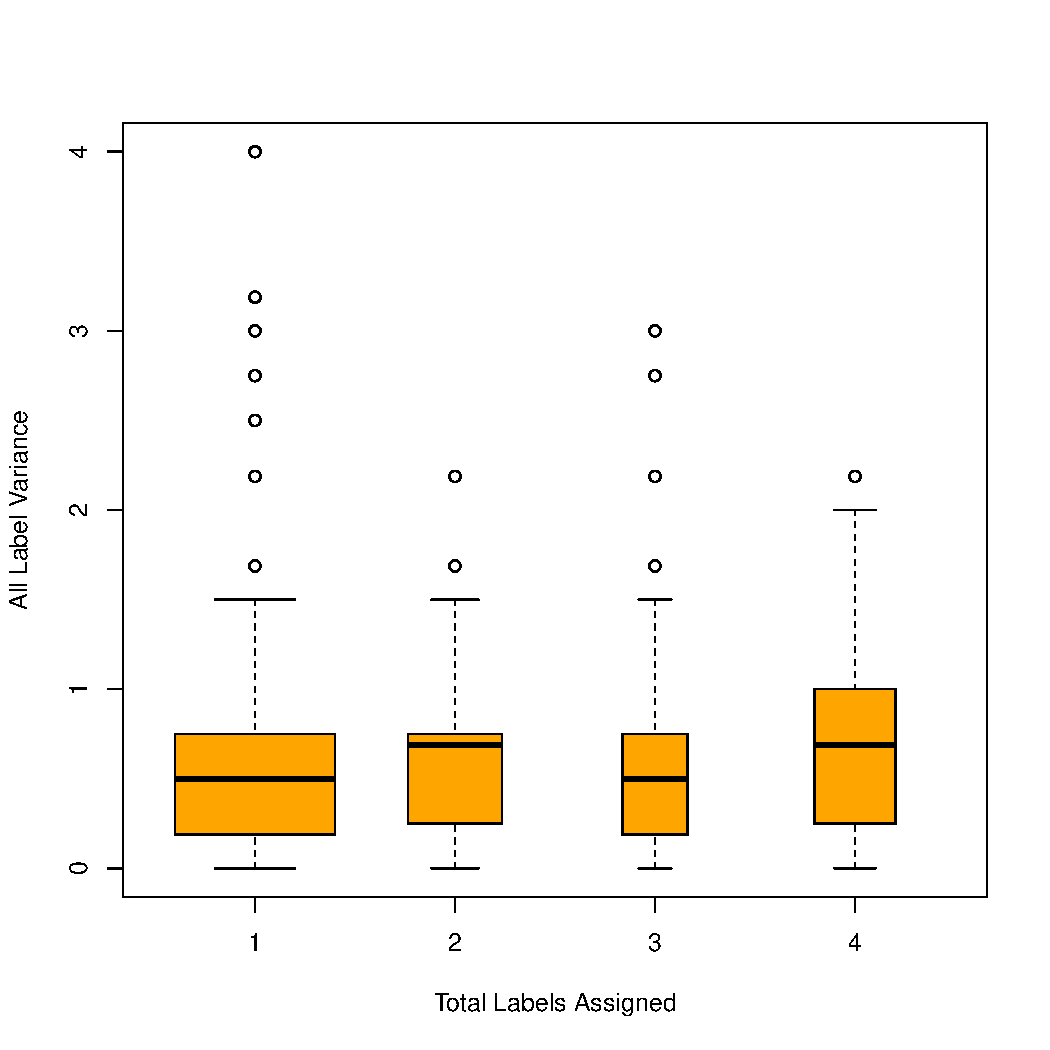
\includegraphics[width=\linewidth]{allvar.pdf}
  \caption[Variance for cases by total labels added]
   { \label{fig: allvar}
Label variances for cases receiving one label, two labels, three labels, and four labels respectively.}
\end{minipage}
\hfill
\begin{minipage}{.45\textwidth}
  \centering
  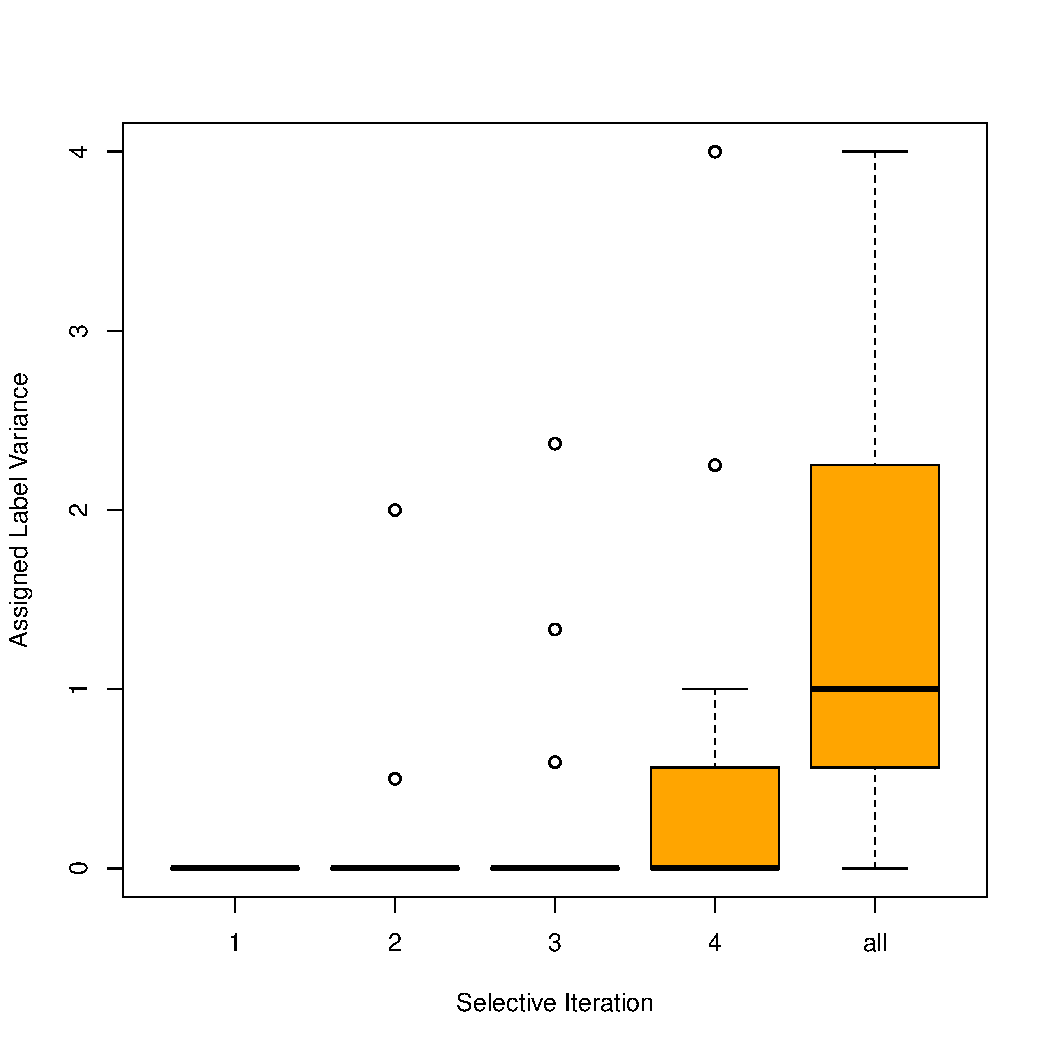
\includegraphics[width=\linewidth]{setvar.pdf}
  \caption[Variance for label sets at selective iterations]
   { \label{fig: setvar}
Label variances at each selective iteration and for all possible labels provided by radiologists.}
\end{minipage}%
\end{figure}

   \subsubsection{Case examples}
    \begin{table}[h]
    \centering
    \captionsetup{width=15cm}
    \caption{Examples of label acquisition cases from the most representative trial with reference truths used at each iteration.} 
    \vfill
    \begin{tabular}{|c|c|c|c|c|c|}
    \toprule
 \multicolumn{1}{|p{2cm}|}{\centering Instance Number} & \multicolumn{1}{|p{2cm}|}{\centering Possible Label Order} & \multicolumn{1}{|p{2cm}|}{\centering Reference at It. 1} & \multicolumn{1}{|p{\textwidth/8}|}{\centering Reference at It. 2} & \multicolumn{1}{|p{2cm}|}{\centering Reference at It. 3} & \multicolumn{1}{|p{2cm}|}{\centering Reference at It. 4}\\
    \midrule
        1 & 1 1 1 1 & 1 & 1 & 1 & 1\\
            \hline
        203 & 3 1 3 1 & 3 & 3 & 3 & 3\\
            \hline
        801 & 3 1 1 1 & 3* & 2* & 1 & 1\\
    \bottomrule
    \end{tabular}
        \caption*{* denotes reference truths that were associated with a misclassification of the case and thus the request of another label.}
  \label{tab:examples}
\end{table}
To give more concrete examples of how our selective iterative method works, Table \ref{tab:examples}shows cases from the most representative trial with extremely high or extremely low all-label variance that demonstrate some of the ways in which the selective iterative method can reduce noise. The most representative trial was the trial with accuracies at each iteration closest to the average accuracy across trials.

Instance 1 is an example of a case in which there was no label uncertainty and the selective method saved resources by only requesting the first label. Since the image features and the label agreed, there was no need to request another label to gain more information.
   
For both instance 203 and 801, which had high variance in radiologist labels, the cost of correct classification (the number of labels requested) was directly affected by the order of label acquisition, which is specific to this trial, since labels are shuffled for every trial. However, they demonstrate the intelligence of the system in reducing the large amount of noise in their labels. For example, instance 203 was consistently classified at a 3 at every iteration because its image features were similar to other cases that were, perhaps with less uncertainty, labeled as 3s. Since the first label acquired was a 3, the case was never misclassified and no additional labels were added, reducing both uncertainty and cost by using only one label. If by the chance of the random permutation the first label for this case had been a 1, the algorithm would have needed more labels (more resources) to reach the same conclusion.

On the other hand, in this trial instance 801 received labels in an order that resulted in a less impressive cost reduction, but still managed to reduce cost and noise over a model that used all four labels indiscriminately. instance 801 was consistently classified as a 1 because of its image features. However, at the first iteration it was labeled as a 3 and misclassified. At the second, it was labeled as a 2 (the mode of ${3,1}$) and again misclassified until the third iteration when it was finally labeled as a 1 (the mode of ${3, 1, 1}$). In this case, cost was reduced by less (three instead of four labels) and uncertainty was either reduced or maintained equal. Importantly, the selective iterative method was able to differentiate well between the cases that needed more information and those that did not.

%%%%%%%%%%%%%%%%%%%%%%%%%%%%%%%%%%%%%%%%%%%%%%%%%%%%%%%%%%%%%
\subsection{Trees}

%-------------
   \begin{figure}[b]
   \begin{center}
   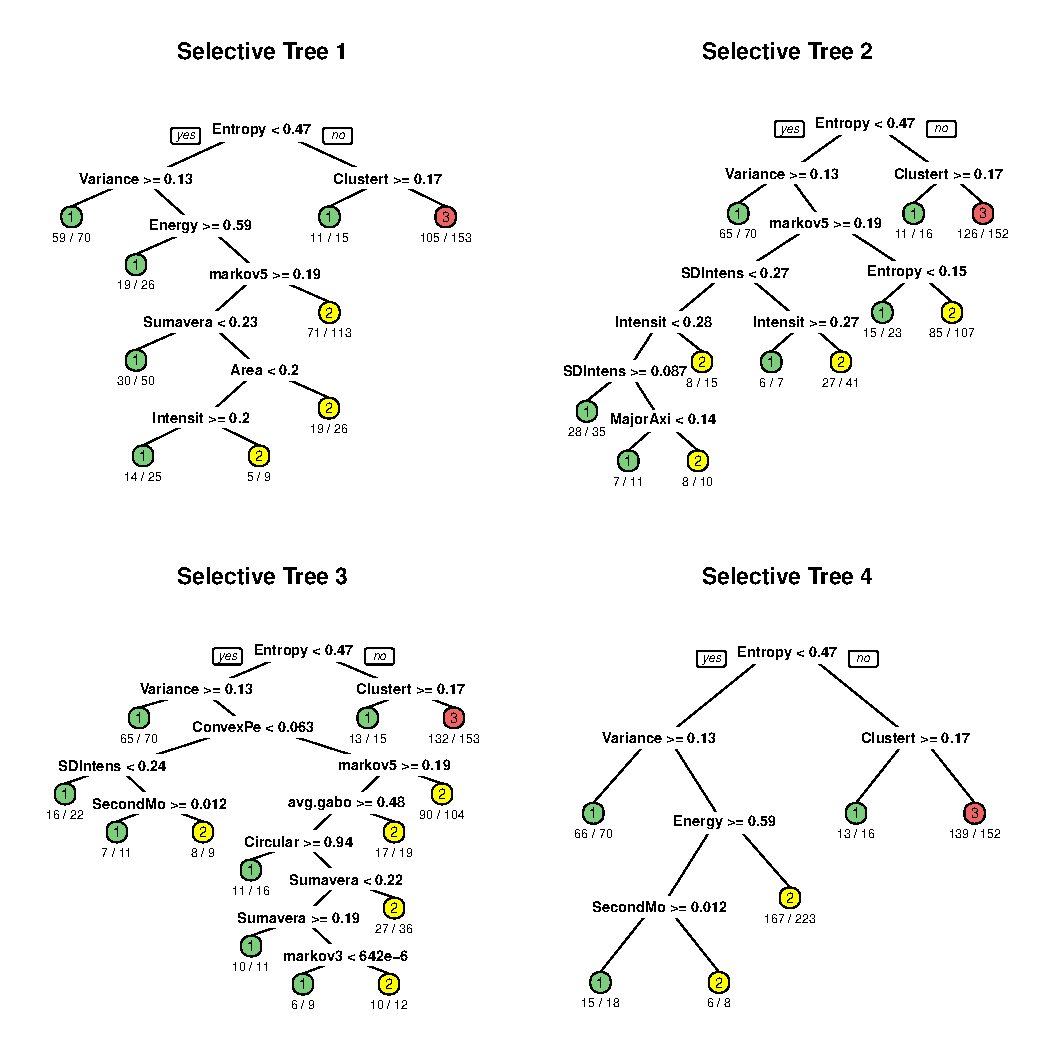
\includegraphics[width = \textwidth]{selectiveTrees.pdf}
   \end{center}
   \caption[Selective Trees]
   { \label{fig: select}
The series of selective trees generated by the most representative trial of the iterative algorithm, numbered by iteration.}
   \end{figure}
 \begin{figure}[h]
   \begin{center}
   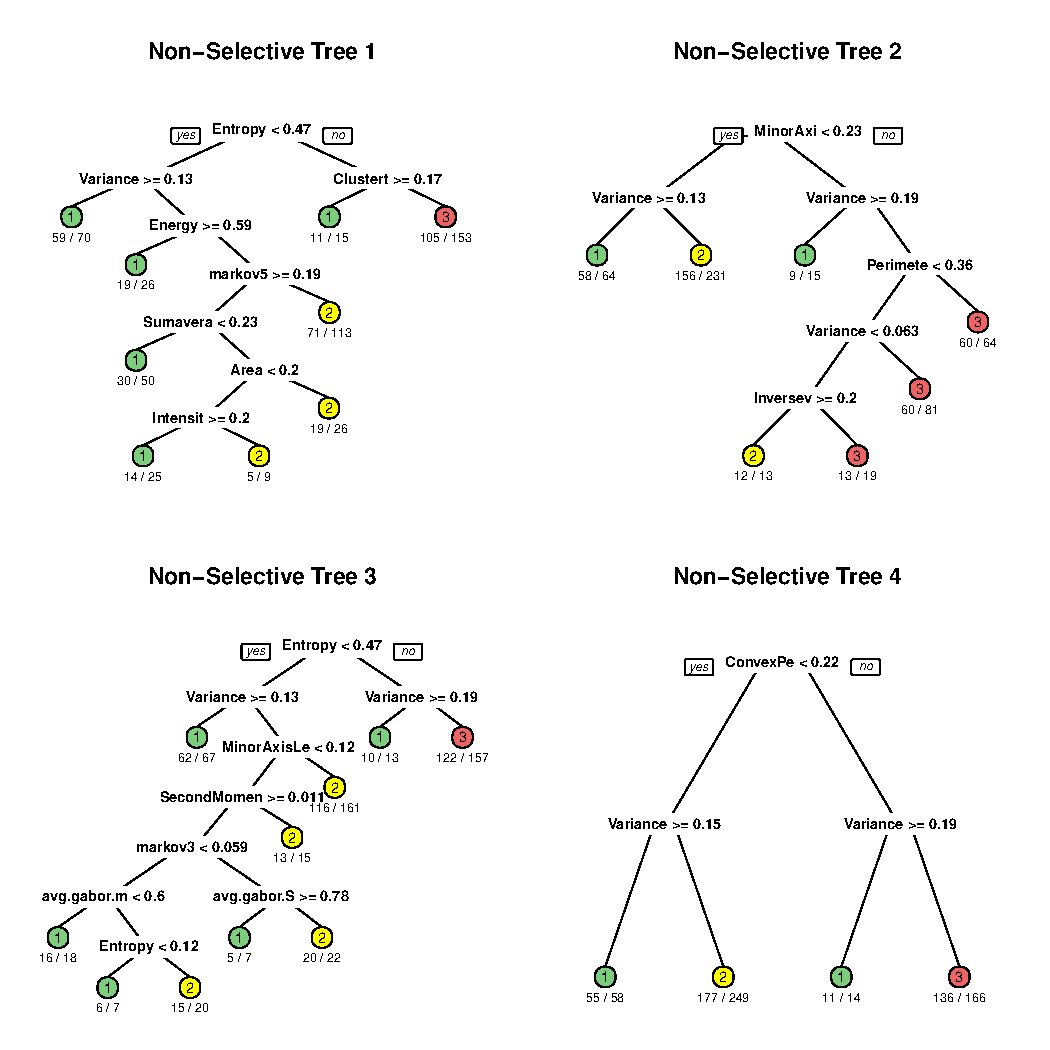
\includegraphics[width = \textwidth]{nonselectiveTrees.pdf}
   \end{center}
   \caption[Non-Selective Trees]
   { \label{fig: nonselect}
The series of non-selective trees generated by the most representative trial of the iterative algorithm, numbered by iteration.}
   \end{figure}
%-------------

In this section we have provided graphical representations of the decision trees produced at each iteration in both the selective and the non-selective iterative method (Figures \ref{fig: select} and \ref{fig: nonselect}) for a deeper look into the changes that the classifiers undergo as labels are added in different ways. Nodules in the green leaves were classified as benign, yellow as unknown, and red as malignant. Accuracy for each particular split can be found just beneath it.

Since within any given trial, the two methods start out with the exact same single label for each case, the trees at the first iteration, like the accuracies at the first iteration, are exactly the same. However, even at the second iteration, the two methods show a prioritization of different image features. For example, the most important split variable in the non-selective tree is not used in the selective tree at all. Importantly, the selective trees show a much more stable feature selection than the non-selective trees. Since decision trees are usually quite unstable, this stability is another sign of the reduction in noise.

%%%%%%%%%%%%%%%%%%%%%%%%%%%%%%%%%%%%%%%%%%%%%%%%%%%%%%%%%%%%%
\section{Conclusion and Future Work}
\label{sec:conclusion}
As we have seen, a selective iterative classification model is preferred when using data with similar constraints to ours (no ground truth, uncertain labels). We have achieved higher than 10\% classification accuracy in the fourth iteration than in previous works’ model using a non-selective approach. This was also accomplished using less than half of the given labels. We have also noted that this method is robust and can be effective when dealing with data that is subject to uncertainty. We believe that this was due to the decreased variability among labels given per case. 
	
Future work will consider expanding this model to then differentiate case difficulty among cases, as in Zamacona et al. \cite{Zamacona13}, by using pattern analysis on misclassifcation strings for each case. 
%%%%%%%%%%%%%%%%%%%%%%%%%%%%%%%%%%%%%%%%%%%%%%%%%%%%%%%%%%%%%
\acknowledgments      
 
A. Riely and K. Sablan were supported by the NSF Medical Informatics (MedIX) REU Program Award No. 1359459.  The image features were extracted by Ronald Niehaus, research assistant in the Medical Informatics Lab at DePaul.

%%%%%%%%%%%%%%%%%%%%%%%%%%%%%%%%%%%%%%%%%%%%%%%%%%%%%%%%%%%%%
%%%%% References %%%%%

\bibliography{report}   %>>>> bibliography data in report.bib
\bibliographystyle{spiebib}   %>>>> makes bibtex use spiebib.bst

\end{document} r